\documentclass[11pt]{article}
\usepackage[margin=0.85in]{geometry}
\usepackage{amsmath,amssymb,booktabs,graphicx,tabularx,array}
\usepackage{microtype,float,caption}
\usepackage[hidelinks]{hyperref}
\hypersetup{pdftitle={ODE-FFN: Progress Report 3},pdfauthor={Zhizhe Zhang}}
\captionsetup{font=small,labelfont=bf,skip=5pt}
\setlength{\parindent}{0pt}
\setlength{\parskip}{5pt}
\setlength{\intextsep}{7pt}
\renewcommand{\arraystretch}{1.14}
\linespread{1.035}
\newcommand{\sw}{\operatorname{SW2}}
\newcommand{\isru}{\operatorname{ISRU}}
\newcommand{\supporttitle}[1]{\section{#1}\vspace{2pt}}
\begin{document}
\begin{center}
{\LARGE\bfseries ODE-FFN: Progress Report 3}\par
\vspace{4pt}
{\large Separating operator sharing from ODE accuracy}\par
\vspace{6pt}
Zhizhe Zhang\quad\textbar\quad NYU Shanghai\par
18 November 2026
\end{center}
\vspace{3pt}

\section{Project and main progress}
This project develops ODE-inspired feedforward networks (FFNs) for flow
matching, starting from a truncated matrix exponential with a shared learned
operator. Our main finding is that sharing improves generation in the tested
stage comparisons, whereas prescribed coefficients and greater ODE solution
accuracy provide no consistent gain. This makes shared nonlinear iteration
the leading architectural hypothesis. We also identify symmetry breaking in
Ring8's fitting--sampling mismatch and analytically predict how changing the
hidden solver changes the complete network output.

Tests use a width-64, three-block velocity MLP. Ring8 has eight equal-weight 2D
Gaussian modes; Product16 is a rotated product of sixteen bimodal factors.
Training uses 20,000 updates, batch~512. Oracle MSE measures field fitting;
sliced Wasserstein distance (SW2) measures generation. Each comparison shares
inputs and eight banks of 4,096 samples. Tables report pooled SW2 within the
named cohort. Image transfer uses the author-derived JiT on CelebA128.

\section{Why better field fitting can give worse samples}
\textbf{Ring8 case study.} Report~2 found that ISRU-D's field MSE improved
between 15k and 20k updates while mode balance deteriorated. We tested whether
the learned field violated the target's 45-degree rotation symmetry. The
intervention averages eight rotated predictions after mapping each velocity
back to the original coordinates. It changes no learned weights.

On rotation-balanced validation states, field error separates into a
symmetry-preserving component and a symmetry-breaking component. From 15k to
20k, the first decreases from $4.955\times10^{-3}$ to $3.256\times10^{-3}$,
while the second increases from $5.745\times10^{-3}$ to $6.532\times10^{-3}$.
Total MSE falls, but the field
becomes more asymmetric. At 20k, enforcing the symmetry lowers pooled SW2 from
0.133 to 0.053 and sector-frequency L1 error from 0.055 to 0.006. Ordinary
Free ISRU and SwiGLU improve too (Table~\ref{tab:symmetry}).
Figures~\ref{fig:trajectories} and~\ref{fig:ringcase} illustrate the trajectories
and generated distributions.
This identifies a shared mode-allocation failure. The projection uses eight
field predictions, so it serves here as a diagnostic intervention.

\textbf{Weight geometry and response.} On Product16 Free ISRU, Muon versus
AdamW raises update stable rank from 4.567 to 32.776, while weight entropy rank
falls from 55.547 to 43.789 and condition number rises from 109.267 to 690.632.
Broad updates need not produce broad, well-conditioned weights
(Table~\ref{tab:ranks}). Matched scaled tanh competes with ISRU
(Table~\ref{tab:response}). A wider eight-response screen likewise finds no
consistent ISRU-specific advantage. This motivates testing the structural
constraints separately from the activation's ODE origin.

\newpage
\section{Which part of the ODE structure contributes?}
\textbf{Two distinct constructions.} In frozen-diagonal ISRU-D, the entrance
state determines $D(h)$ once; the block applies a Taylor polynomial in
$A(h)=PD(h)$. D rescales each coordinate; K denotes the highest Taylor power.
In the state-flow model, the response is recomputed as the
hidden state evolves:
\begin{equation}
\frac{dy}{ds}=f(y)=Pq(y),\qquad
q_i(y)=\frac{y_i}{\sqrt{1+1.2y_i^2}},\qquad y(0)=h.
\label{eq:stateflow}
\end{equation}
The internal duration is one. This hidden time $s$ is separate from the
flow-matching time supplied to the complete network. Four midpoint substeps
use eight applications of P. Both constructions have the same first-order
increment, but their higher-order terms differ because the second updates
the response along the path.

\textbf{Sharing P.} We tested whether using one stationary operator matters
by allowing the four stages to learn different matrices. The shared and
released models start from the same function, receive the same minibatches,
and use identical matrix work. Releasing stages adds parameters. At 20k,
shared/released pooled SW2 is 0.091/0.111 on Ring8 and 0.064/0.073 on
Product16; sharing wins all eight paired banks on each task
(Table~\ref{tab:sharing}). On Product16 the released model fits the field
slightly better, so its worse generation is not explained by poorer fitting.

The release also changes optimization coordinates: the initial implementation
writes stage matrices as P plus learned offsets. We therefore tested a
mean-preserving representation of the same released function class. Its SW2
is 0.104/0.072 on Ring8/Product16. The Ring8 difference from sharing is
unresolved across banks; Product16 still favors sharing. This establishes a
useful shared-operator constraint in the tested family while exposing an
optimization effect in the original release comparison.

\textbf{Expansion and stage coefficients.} To test the necessity of the
prescribed coefficients, we made the higher Taylor terms learnable, starting
from the exact original polynomial. Generation remains close to the fixed
version: Ring8 SW2 is 0.088 versus 0.089, and Product16 is 0.056 versus 0.055.
Freeing midpoint stage coefficients likewise gives similar sampling
(Table~\ref{tab:coefficients}). The learned coefficients are active: resetting
them after training changes the output. However, independently trained fixed
and free models perform similarly. The free-stage version also loses the
fixed midpoint method's near-second-order convergence. Using a mechanism
during training therefore does not establish its necessity for generation.

\textbf{More accurate solves.} We next replaced four midpoint steps by two
classical RK4 steps. Parameter count, initialization, data and optimizer are
unchanged; both methods use eight P applications per local solve. Measured
against high-accuracy solutions of each learned field, RK4 reduces normalized
hidden squared error about 46-fold on Ring8 and 22-fold on Product16. Yet
confirmation SW2 changes from 0.091 to 0.091 and from 0.064 to 0.065,
respectively (Figure~\ref{fig:solver}). Accurate local ODE solution is thus
insufficient to explain good generation in this comparison. The next question
is how the hidden numerical difference reaches the complete output field.

\newpage
\section{From hidden numerical error to generation}
\textbf{Predicting the output change.} We derived a correction from the
midpoint and RK4 numerical defects, then propagated it through all six local
flows and the unchanged downstream network. For each local flow, the
response calculation follows
\begin{equation}
\frac{dy}{ds}=f(y),\qquad
\frac{dz}{ds}=J_f(y)z+G(y),\qquad z(0)=0.
\label{eq:response}
\end{equation}
Here $G$ is the solver-derived forcing and $z$ predicts the hidden-state
change. The correction uses the learned matrices and response derivatives;
no scale is fitted to the measured output difference.

Across four trained models and two 4,096-input streams, the complete-field
prediction score is 0.957--0.983. The score is one minus prediction squared
error divided by the squared error of predicting no change. Product16
RK4-trained weights score 0.962 on both streams, with relative RMS error
0.196 and vector alignment 0.987 (Figure~\ref{fig:forecast}). This gives a
quantitative connection from the local ODE calculation to the actual network.

\textbf{Field fitting and generation remain distinct.} With those fixed
Product16 RK4 weights, switching inference to midpoint slightly worsens
oracle field MSE; the analytic correction predicts that increase. Nevertheless,
generation improves. The effect survives outer Heun refinement through 2,048
steps: pooled SW2 decreases from 0.053 to 0.049 on selection and from 0.048 to
0.045 on confirmation, with all eight banks improving in each stream. The
field-response prediction is complete; a high-resolution analytic forecast
of the final distribution remains unfinished.

\textbf{Practical comparison.} All models use the same source, target and
direction arrays. At Heun2048,
native midpoint state flow reaches confirmation SW2 0.068 on Ring8 versus
0.091 for Free ISRU and 0.105 for SwiGLU. On Product16 it reaches 0.047 versus
0.051 and 0.034. The Ring8 pooled ordering favors state flow, although most
adjusted paired-bank intervals include zero. State flow uses about four times
Free ISRU's dense forward matrix work (Table~\ref{tab:ordinary}).

On CelebA128 at 160 epochs,
native SwiGLU achieves FID50k 24.304, versus 27.789 for parameter-matched
ISRU-D K1 and 28.083 for K8. Native leads at every shared checkpoint
(Table~\ref{tab:image}). These image blocks use frozen entrance diagonals;
the refreshed state-flow model has not been tested in this image comparison.

\section{Hypothesis for the next two weeks}
Our final-stage hypothesis is that shared nonlinear iteration improves
quality per training computation, with midpoint structure adding value beyond
plain recurrence. On Ring8 and Product16, compare midpoint with a tied
residual block, Free ISRU and SwiGLU. The residual block uses the same response
$Pq(y)$ in eight updates $y\leftarrow y+Pq(y)/8$, without midpoint evaluations.
Match cumulative forward, backward and optimizer work; retain seed~0,
common sample banks and mode-balance measurements.

If tied residual iteration matches midpoint, retain the simpler shared
architecture. If midpoint leads at matched cost, its stage structure becomes
the architectural contribution. If ordinary FFNs catch up, the current gain
is a computation trade-off. Only a candidate with a demonstrated quality--cost
advantage proceeds to CelebA. These comparisons are planned, not yet run.
\label{main:end}

\clearpage
\appendix
\supporttitle{Weight geometry, response and symmetry}
\begin{table}[H]
\centering\small
\begin{tabular}{@{}lrrrr@{}}
\toprule
Model / optimizer & \shortstack{Update\\stable rank} & \shortstack{Weight\\stable rank} & \shortstack{Weight\\entropy rank} & \shortstack{Weight\\condition no.}\\
\midrule
Free ISRU / AdamW & 4.567 & 13.018 & 55.547 & 109.267\\
Free ISRU / Muon & 32.776 & 10.525 & 43.789 & 690.632\\
ISRU-D / AdamW & 1.648 & 9.703 & 47.510 & 885.527\\
ISRU-D / Muon & 32.905 & 12.379 & 46.674 & 1368.710\\
\bottomrule
\end{tabular}
\caption{Product16 at 20k updates; means over six learned matrices. The matrix learning rates are 0.0003 for AdamW and 0.02 for Muon; other parameters use AdamW 0.0003.}
\label{tab:ranks}
\end{table}
\begin{table}[H]
\centering\small
\begin{tabular}{@{}llrr@{}}
\toprule
Task & Response & Field MSE ($\times10^{-3}$) & Pooled SW2\\
\midrule
Ring8 & ISRU & 9.773 & 0.133\\
Ring8 & Scaled tanh & 9.611 & 0.140\\
Product16 & ISRU & 16.059 & 0.072\\
Product16 & Scaled tanh & 16.489 & 0.070\\
\bottomrule
\end{tabular}
\caption{Matched K1 response comparison at 20k updates, AdamW 0.0003 and Heun128. Scaled tanh matches the slope at zero, odd symmetry and saturation of ISRU; parameters, initialization and data stream are held fixed. Lower is better.}
\label{tab:response}
\end{table}

\begin{figure}[H]
\centering
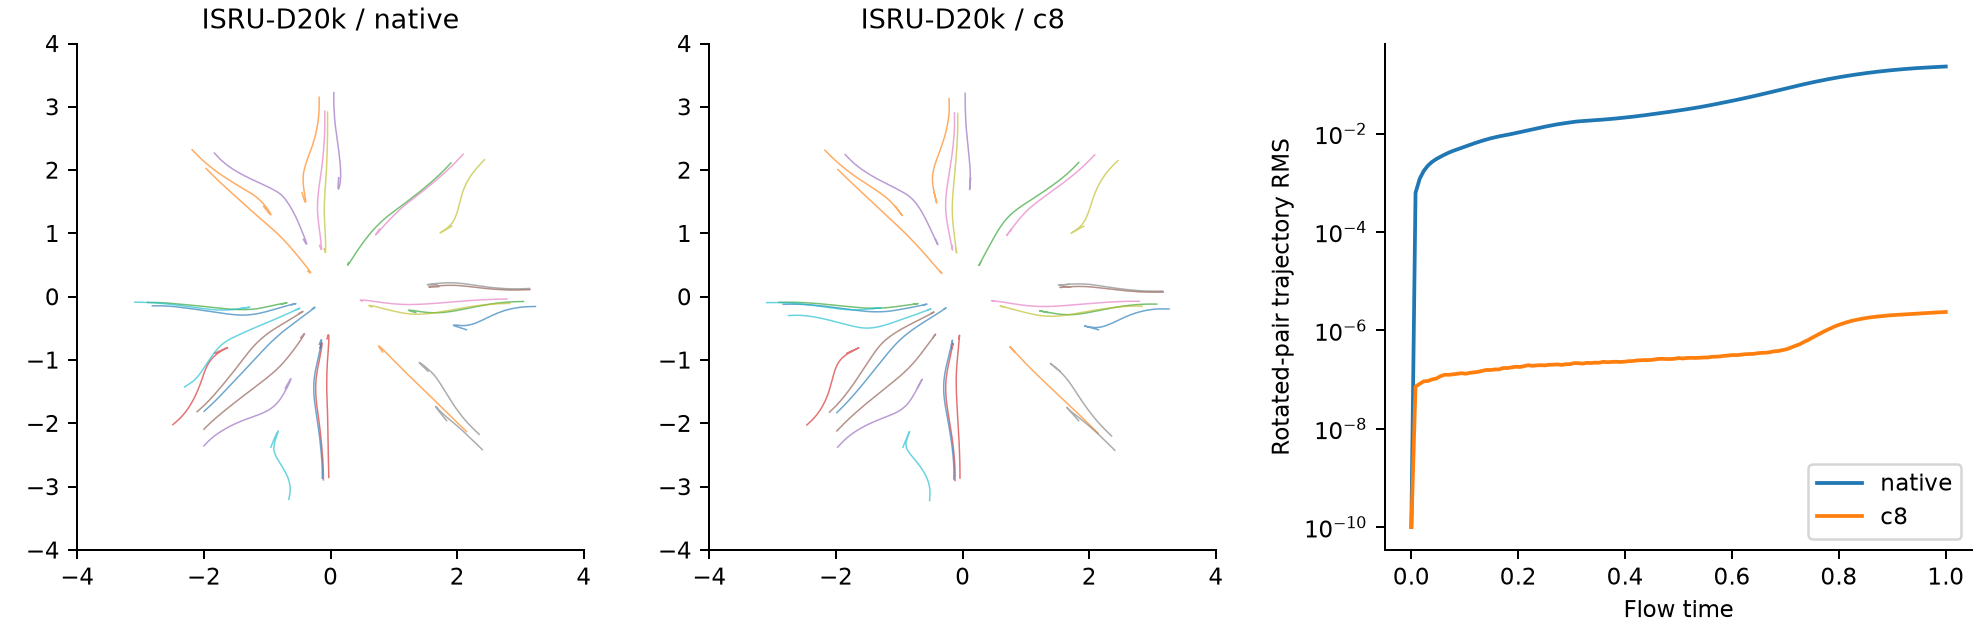
\includegraphics[width=\textwidth]{figures/ring8-trajectories.png}
\caption{Paired trajectories from the recorded symmetry diagnosis. Rotated
initial states need not give rotated native trajectories; C8 projection
enforces the discrete rotation relation. These are fixed examples from the
recorded checkpoint evaluations.}
\label{fig:trajectories}
\end{figure}

\clearpage
\supporttitle{Ring8 checkpoint case study}
\begin{figure}[H]
\centering
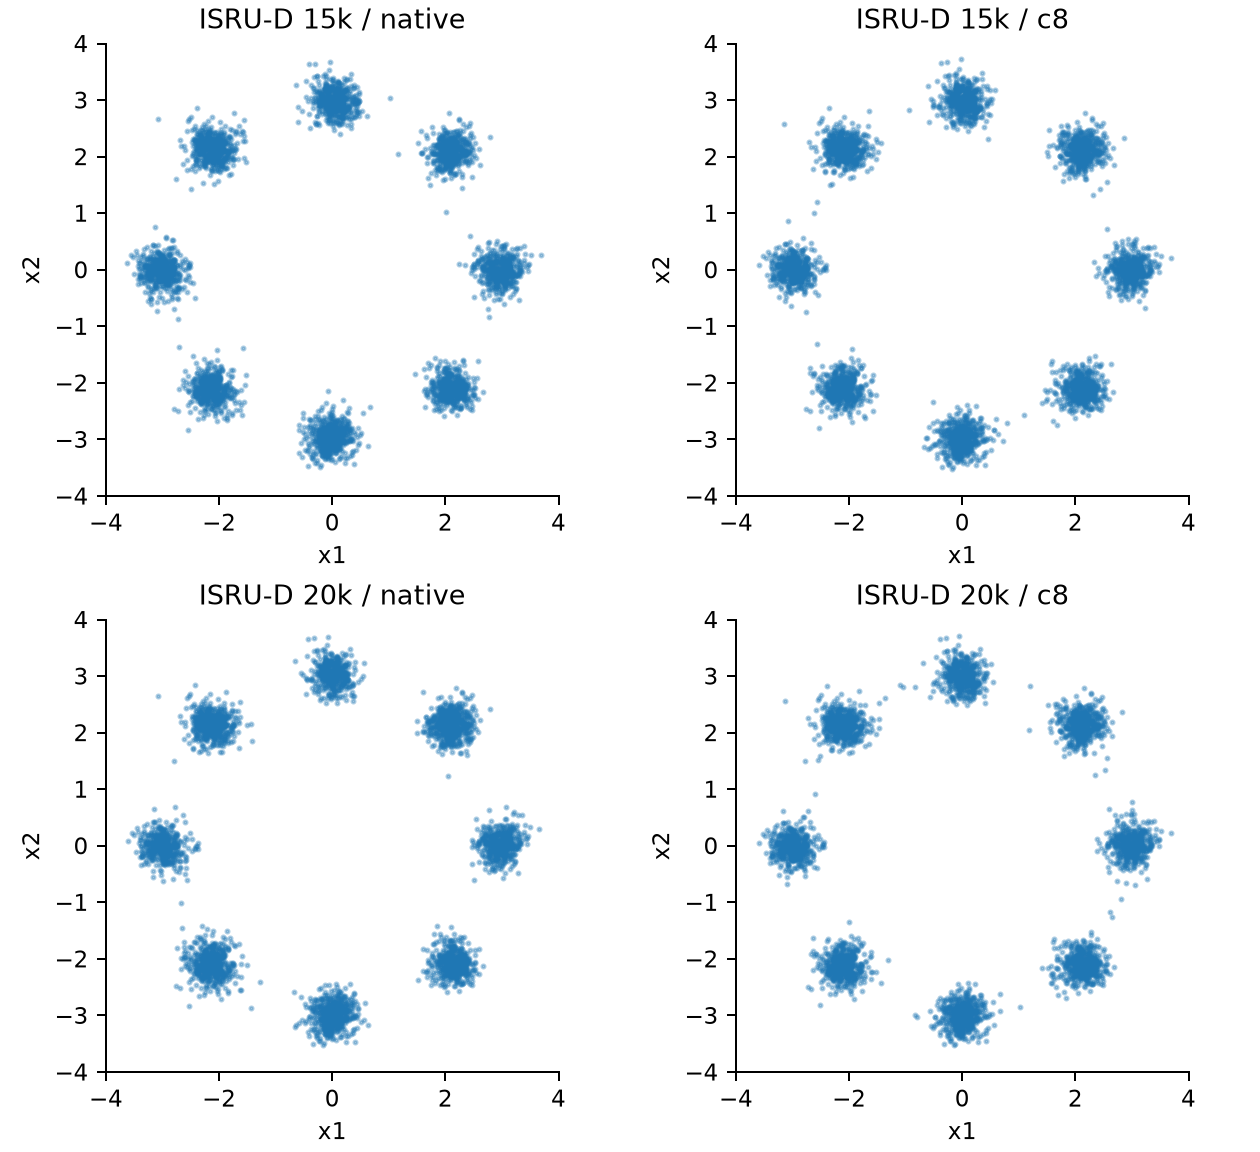
\includegraphics[width=0.95\textwidth]{figures/ring8-samples.png}
\caption{The same ISRU-D checkpoints before and after C8 projection. Top:
15k updates; bottom: 20k. Each panel uses the same fixed display indices from
its saved generated samples. Visible clusters alone do not establish balanced
mode probabilities; Table~\ref{tab:symmetry} quantifies the pooled imbalance.}
\label{fig:ringcase}
\end{figure}
\begin{table}[H]
\centering\small
\begin{tabular}{@{}lrrrr@{}}
\toprule
Model & \shortstack{Native\\SW2} & \shortstack{C8\\SW2} & \shortstack{Native\\sector L1} & \shortstack{C8\\sector L1}\\
\midrule
ISRU-D & 0.133 & 0.053 & 0.055 & 0.006\\
Tanh-D & 0.140 & 0.052 & 0.055 & 0.007\\
Free ISRU & 0.145 & 0.052 & 0.074 & 0.006\\
SwiGLU64 / Muon & 0.157 & 0.053 & 0.063 & 0.007\\
\bottomrule
\end{tabular}
\caption{Ring8 at 20k, Heun128, eight common 4,096-sample banks pooled. Sector L1 is deviation from equal mode frequencies. C8 uses eight rotated predictions per field evaluation. Its benefit occurs in ordinary and ODE-inspired models. Lower is better.}
\label{tab:symmetry}
\end{table}


\clearpage
\supporttitle{Controls on the ODE structure}
\begin{table}[H]
\centering\small
\begin{tabular}{@{}lrr@{}}
\toprule
Operator design & Ring8 SW2 & Product16 SW2\\
\midrule
Shared P & 0.091 & 0.064\\
Independent stages & 0.111 & 0.073\\
Mean-preserving stage release & 0.104 & 0.072\\
\bottomrule
\end{tabular}
\caption{20k, Heun128; all rows use the same banks and eight P applications per local solve. Shared models have 56,706/58,512 parameters on Ring8/Product16; released models have 130,434/132,240. The mean-preserving and original releases have the same function class. This is a fixed-matrix-work comparison.}
\label{tab:sharing}
\end{table}
\begin{table}[H]
\centering\small
\begin{tabular}{@{}lrr@{}}
\toprule
Coefficient design & Ring8 SW2 & Product16 SW2\\
\midrule
Fixed Taylor K8 & 0.088 & 0.056\\
Free Taylor coefficients & 0.089 & 0.055\\
Fixed midpoint stages & 0.071 & 0.052\\
Free midpoint stages & 0.071 & 0.052\\
\bottomrule
\end{tabular}
\caption{20k confirmation, Heun128. Each free-coefficient model starts with the same function as its fixed counterpart and retains its P applications. The free Taylor/stage variants add 42/24 scalar parameters. This cohort differs from Table~\ref{tab:sharing}; compare rows within this table.}
\label{tab:coefficients}
\end{table}

\begin{figure}[H]
\centering
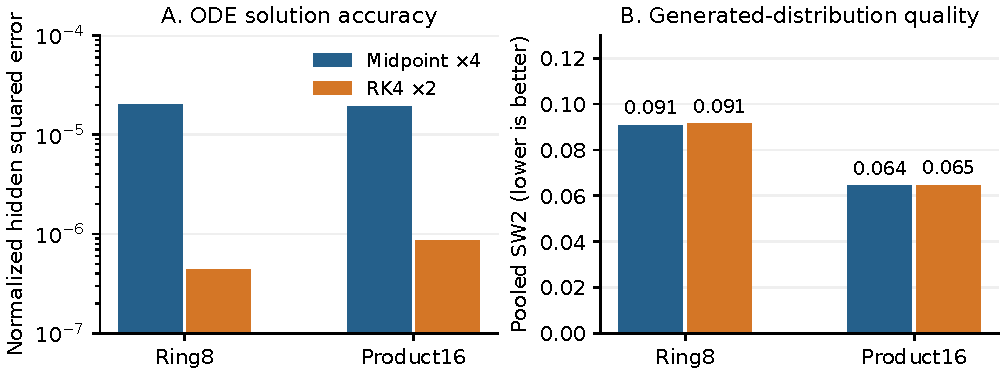
\includegraphics[width=\textwidth]{figures/solver-accuracy-quality.pdf}
\caption{Equal-matrix-work midpoint/RK4 training. Left: normalized hidden
squared error relative to each learned field's high-accuracy solution
(log scale). Right: confirmation pooled SW2 on the same banks. Large numerical
accuracy improvements do not produce a generation gain.}
\label{fig:solver}
\end{figure}

\clearpage
\supporttitle{Output prediction and practical comparisons}
\begin{figure}[H]
\centering
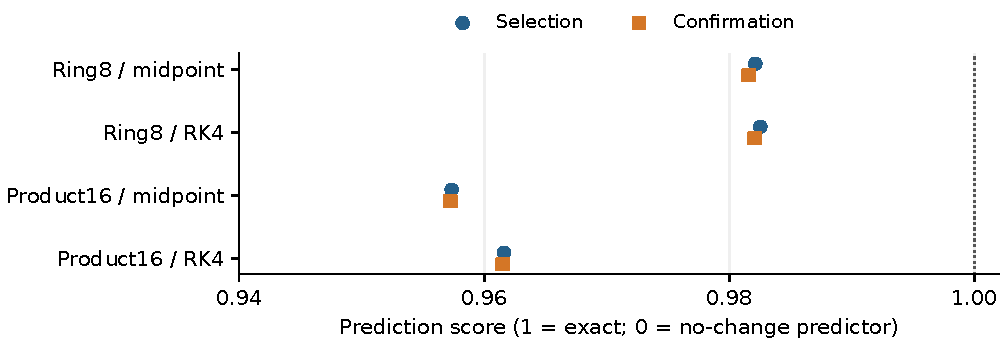
\includegraphics[width=\textwidth]{figures/field-forecast.pdf}
\caption{Unfitted prediction of the complete solver-induced field change.
Both evaluation streams are shown for every trained model. A score of one is
exact prediction; zero is the no-change predictor. The horizontal scale is
restricted to show differences among the qualified results. These scores
measure output-field prediction, not generated-distribution quality.}
\label{fig:forecast}
\end{figure}
\begin{table}[H]
\centering\small
\begin{tabular}{@{}lrrrr@{}}
\toprule
Model & \shortstack{Ring8\\selection} & \shortstack{Ring8\\confirmation} & \shortstack{Product16\\selection} & \shortstack{Product16\\confirmation}\\
\midrule
State flow / midpoint & 0.076 & 0.068 & 0.053 & 0.047\\
Free ISRU / AdamW & 0.096 & 0.091 & 0.051 & 0.051\\
SwiGLU reference & 0.105 & 0.105 & 0.035 & 0.034\\
\bottomrule
\end{tabular}
\caption{Pooled SW2, Heun2048, eight 4,096-sample banks per stream. State flow and Free ISRU use AdamW 0.0003; Ring8 SwiGLU64 uses Muon 0.02 and Product16 SwiGLU192 uses AdamW 0.0003. State/Free dense forward MACs are 227,648/55,616 on Ring8 and 229,440/57,408 on Product16. These are matrix-work counts, not total training FLOPs.}
\label{tab:ordinary}
\end{table}
\begin{table}[H]
\centering\small
\begin{tabular}{@{}rrrr@{}}
\toprule
Epoch & Native SwiGLU & Wide ISRU-D K1 & Wide ISRU-D K8\\
\midrule
100 & 35.918 & 37.925 & 38.136\\
120 & 29.476 & 32.502 & 32.851\\
140 & 25.986 & 29.629 & 30.082\\
160 & 24.304 & 27.789 & 28.083\\
\bottomrule
\end{tabular}
\caption{CelebA128 standard FID50k. Native has 130,405,632 parameters; both widened candidates have 130,402,560. The protocol uses EMA 0.9999, Heun50, CFG0 and the same reference. All three completed 160 epochs. These are frozen-diagonal image blocks, not the refreshed state-flow model.}
\label{tab:image}
\end{table}

\vspace{4pt}
{\small Tables, source bindings and plotting scripts:
\href{https://github.com/Joni-z/ODE-FFN/tree/main/reports/report3}{github.com/Joni-z/ODE-FFN, reports/report3}.}
\end{document}
